%%---------------------------------------------------------------------------%%
%% dtk_scaling_study.tex
%% Stuart R. Slattery
%% Tue Jun 26 09:16:04 2012
%% Copyright (C) 2008-2010 Oak Ridge National Laboratory, UT-Battelle, LLC.
%%---------------------------------------------------------------------------%%
\documentclass[note]{TechNote}
\usepackage[centertags]{amsmath}
\usepackage{amssymb,amsthm}
\usepackage[mathcal]{euscript}
\usepackage{tabularx}
\usepackage{cite}
\usepackage{c++}
\usepackage{tmadd,tmath}

%%---------------------------------------------------------------------------%%
%% DEFINE SPECIFIC ENVIRONMENTS HERE
%%---------------------------------------------------------------------------%%
%\newcommand{\elfit}{\ensuremath{\operatorname{Im}(-1/\epsilon(\vq,\omega)}}
%\newcommand{\vOmega}{\ensuremath{\ve{\Omega}}}
%\newcommand{\hOmega}{\ensuremath{\hat{\ve{\Omega}}}}

%%---------------------------------------------------------------------------%%
%% BEGIN DOCUMENT
%%---------------------------------------------------------------------------%%
\begin{document}

%%---------------------------------------------------------------------------%%
%% OPTIONS FOR NOTE
%%---------------------------------------------------------------------------%%

\refno{RNSD-00-000}
\subject{Data Transfer Kit Scaling Study}

%-------HEADING
\TIname{Reactor and Nuclear Systems Division}
\groupname{Radiation Transport Group}
\from{Stuart R. Slattery}
\date{\today}
%-------HEADING

\audience{\email{Stuart Slattery}{uy7@ornl.gov},
          \email{Thomas Evans}{tme@ornl.gov},
          \email{Greg Davidson}{gqe@ornl.gov},
          \email{John Turner}{jtd@ornl.gov},
         }

%%---------------------------------------------------------------------------%%
%% BEGIN NOTE
%%---------------------------------------------------------------------------%%

\opening

\begin{abstract}
  The Data Transfer Kit (DTK) is a software package designed to
  provide parallel grid transfer services for arbitrary physics
  components. At the core of the DTK design is the concept of the
  geometric rendezvous. The rendezvous algorithm provides a means to
  geometrically correlate two meshes that may be arbitrarily
  decomposed in a parallel simulation. By repartitioning both meshes
  such that they have the same geometric domain on each parallel
  process, efficient and load balanced search operations and field
  evaluations can be performed at a desirable algorithmic time
  complexity with low communication overhead relative to other types
  of mapping algorithms. An initial implementation of the rendezvous
  algorithm has been completed in DTK and this document gives the
  results of initial scaling studies performed on the Jaguar system at
  ORNL. New data has been included to show improvements over the
  previous scaling studies.
\end{abstract}

%%---------------------------------------------------------------------------%%
\section{Introduction}
A typical use case of DTK is searching a mesh with a set of points and
applying field data to those points. For this use case, a scaling
study of the initial DTK implementation of the rendezvous algorithm
for data transfer was performed utilizing the Jaguar system. For each
study, a tri-linear hexahedron mesh was generated and decomposed
across the parallel domain. Figure~\ref{fig:mesh_partition} shows an
example of a mesh partition used in the scaling studies. Each
partition had one element in the z direction while the x and y
directions were varied to produce the desired number of elements in
the partition. All partitions in each scaling study are square. This
mesh is searched with random points generated by sampling the x and y
directions across the global mesh domain.  By striding the random
number seed used to generate the point coordinates, each process will
have a unique set of random points it is searching for. For each
scaling study, every process generated the same number of random
points as the number of elements on that process, ensuring that a
dense, all-to-all communication operation will be required for mapping
and data transfer. Once the points are mapped to the mesh, the data
transfer routine applies the process rank in which they were found and
transfers it back to the original owning process for the point. In
this way, because of the simple partitioning used for the scaling
studies, the results of the data transfer to the random points can be
independently verified by checking the applied data against the
expected mesh process rank.

\begin{figure}[htpb!]
  \centering
  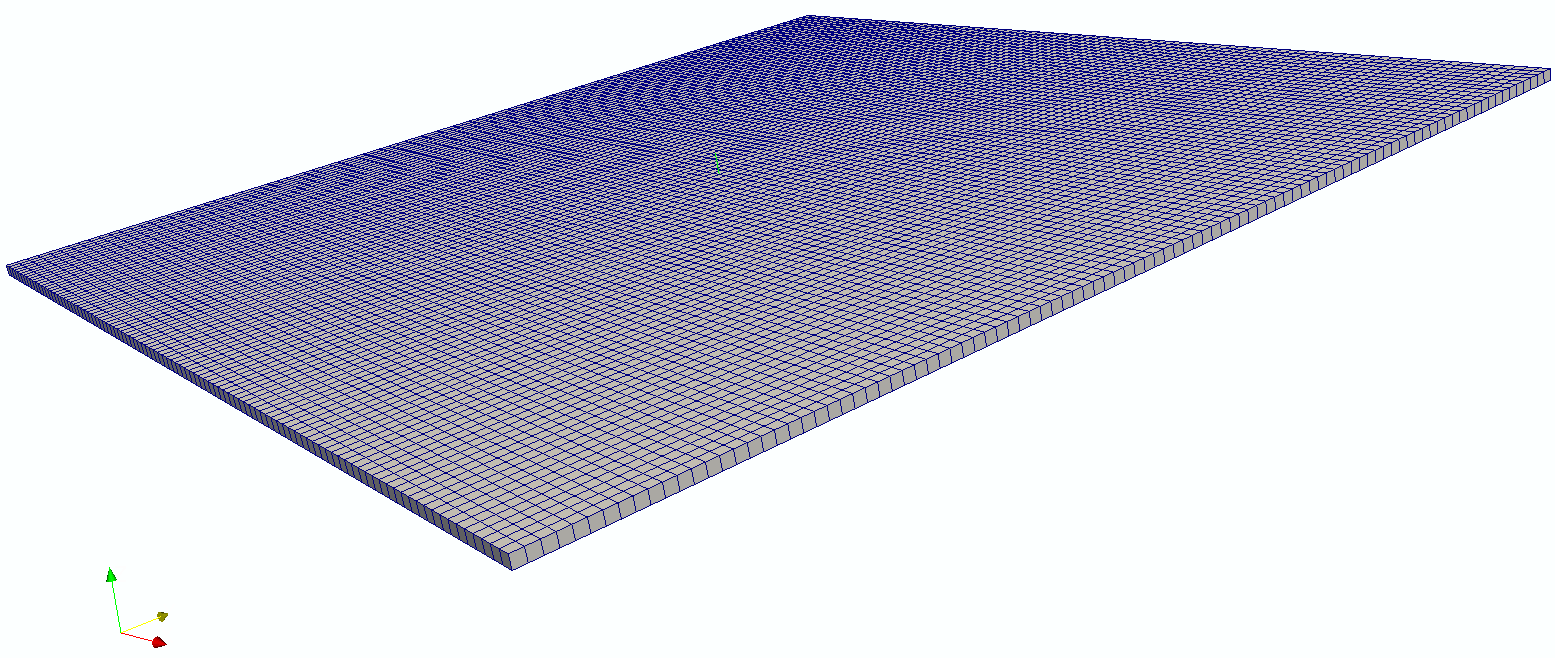
\includegraphics[width=5.5in]{mesh.png}
  \caption{\sl Local mesh partition for scaling studies. This
    particular mesh partition has 1.0E4 tri-linear hexahedrons.}
  \label{fig:mesh_partition}
\end{figure}

Three scaling variations were investigated. A weak scaling study was
performed by fixing the problem size per core and increasing the
number of cores used. A strong scaling study was performed by fixing
the total problem size while increasing the number of cores
used. Finally, a study where the number of cores was fixed while
increasing the total problem size per core was also investigated.

%%---------------------------------------------------------------------------%%
\section{Weak Scaling}
For the weak scaling study, the number of hexahedrons per partition
was fixed to 1.0E4 and the number of random points generated per
partition also fixed to 1.0E4. The number of cores used varied from 16
to 65,536. Figure~\ref{fig:weak_scaling} gives the results of the weak
scaling study. It is clear from the weak scaling study that at high
numbers of processors communication latency begins to dominate for
this dense all-to-all problem as described above. However, it is worth
noting that once the mapping is complete, wall time for the actual
transfer of the data is several orders of magnitude less.

\begin{figure}[htpb!]
  \centering
  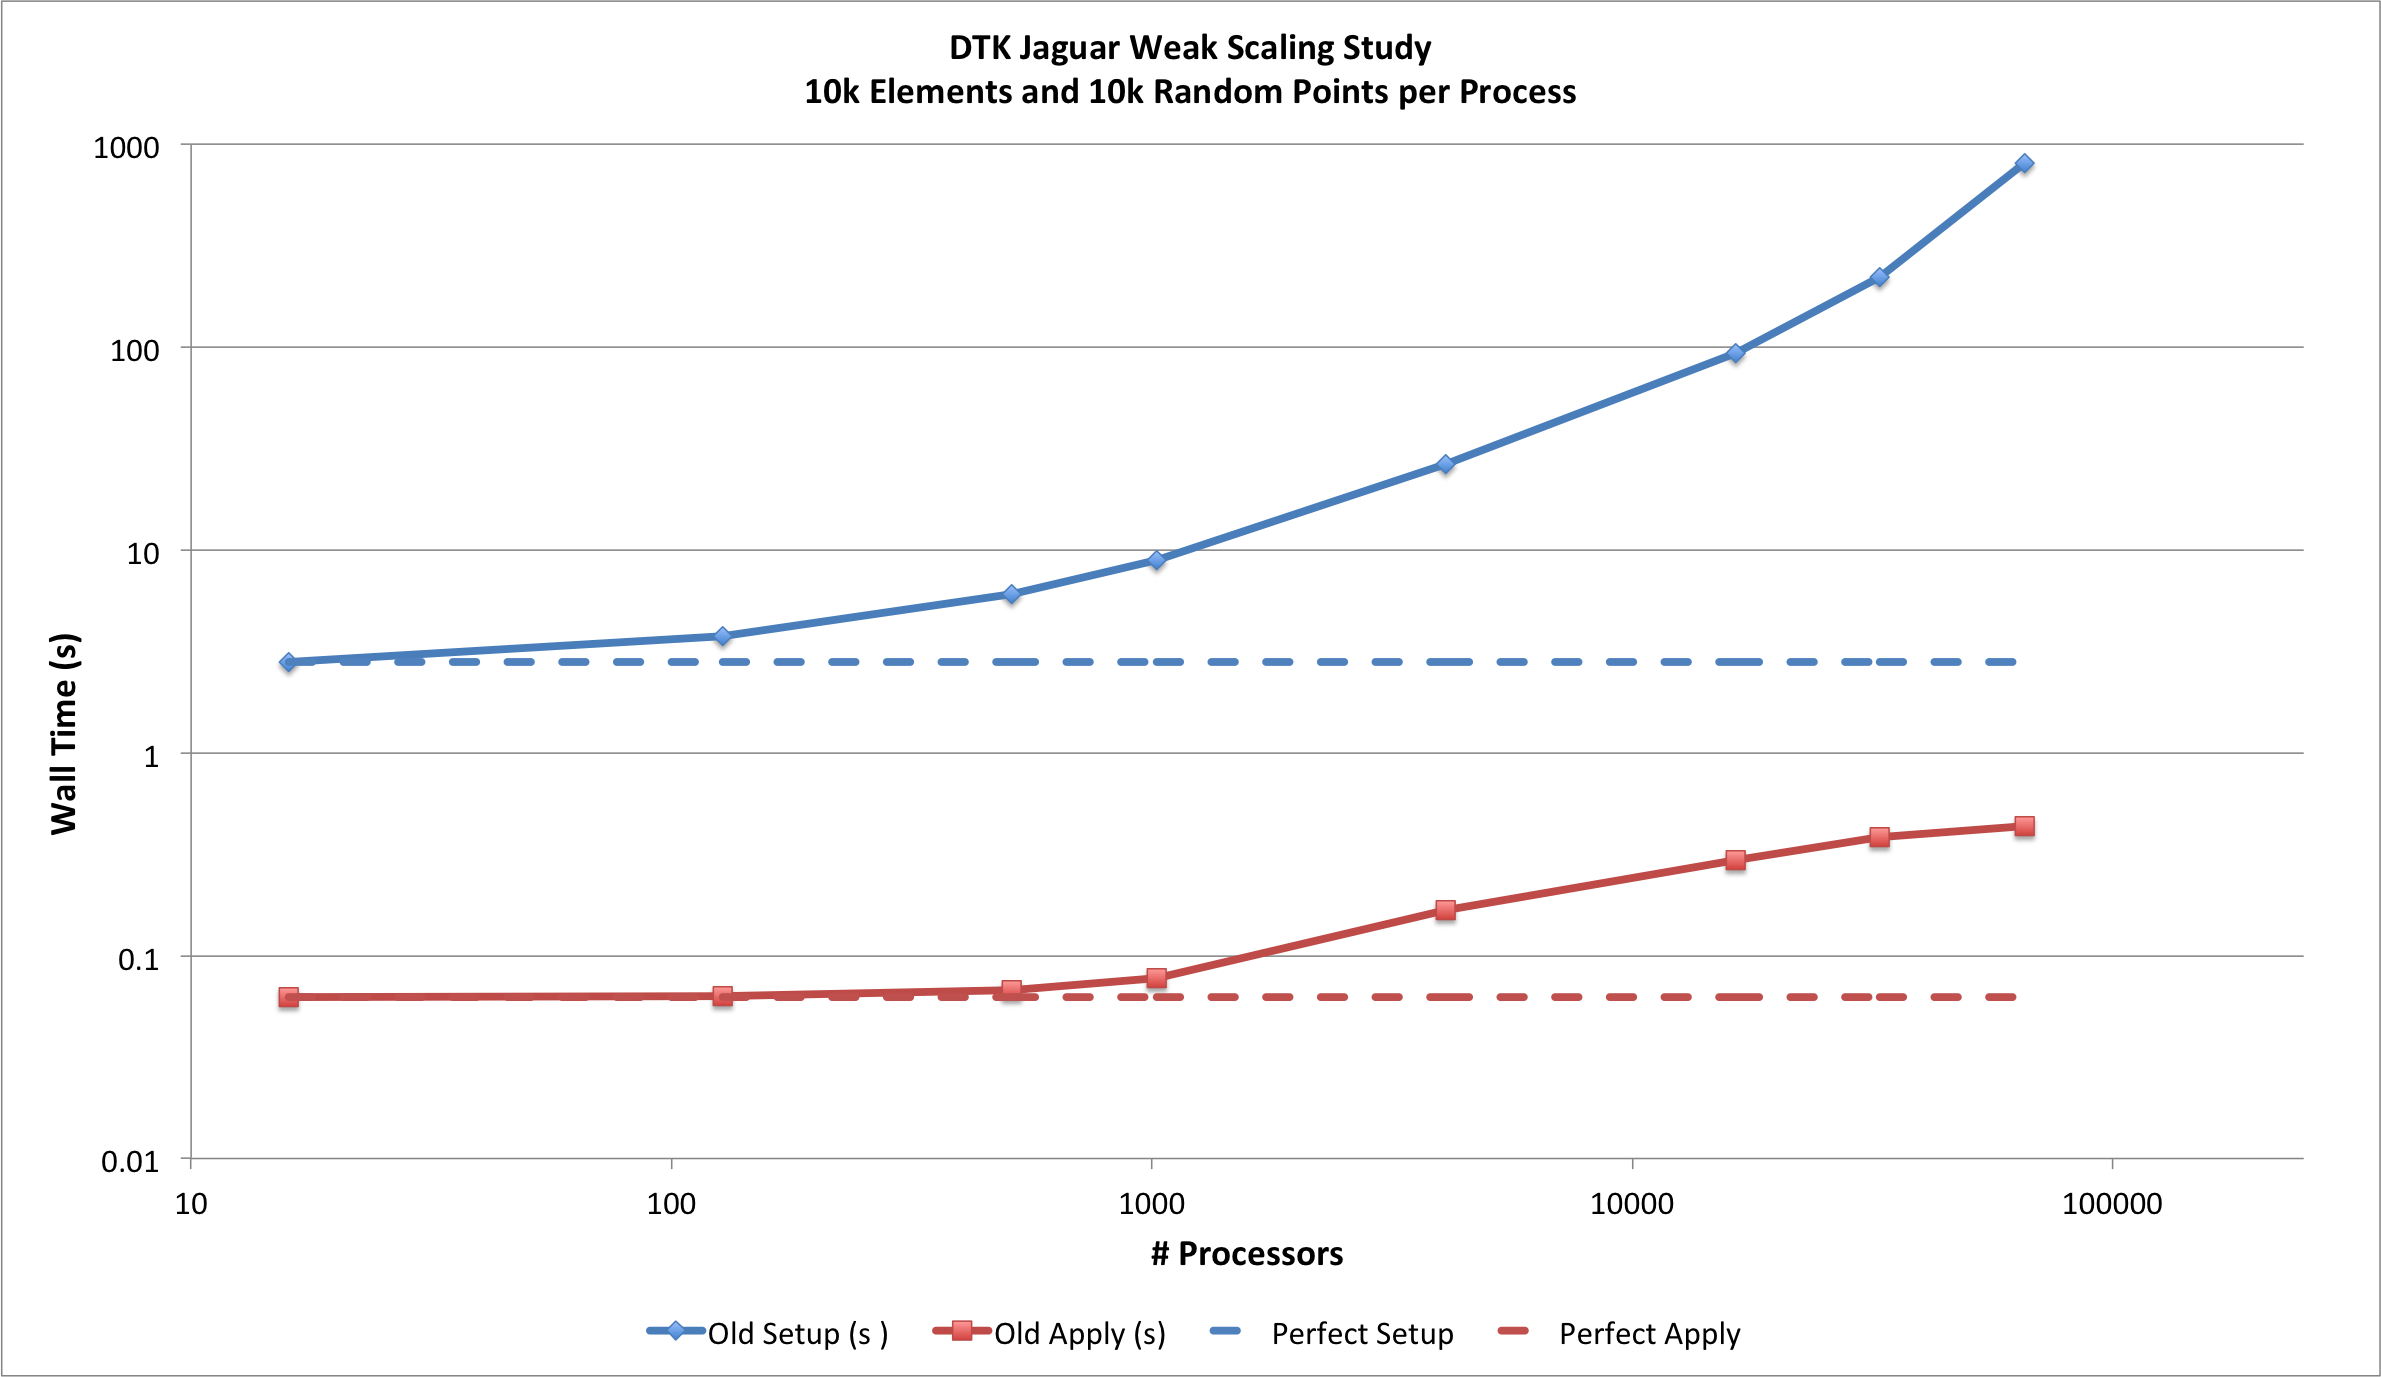
\includegraphics[width=5.5in]{WeakScaling.png}
  \caption{\sl Weak scaling study results. The blue curve reports the
    wall time to generate the mapping (setup) vs. number of processors
    while the red curve reports the wall time to transfer the data
    (apply) vs. number of processors. The dashed lines give perfect
    weak scaling. Note that both axes are on a logarithmic scale. }
  \label{fig:weak_scaling}
\end{figure}

Table~\ref{tab:weak_scaling}. Gives the raw data for the weak scaling
study. We note here that both the setup time (mapping) and the apply
time (data transfer) are relatively load balanced with average compute
times reported near the maximum compute time. In addition it should be
noted that for even the largest case at 65,536 cores the wall time is
not prohibitively large with the setup routine requiring approximately
13.6 minutes and the apply routine requiring less than half a second.

The efficiency values for the apply and setup routines are also
reported in table~\ref{tab:weak_efficiency} with the 16 core case used
as the reference computation. In correlation with the data presented
in table~\ref{tab:weak_scaling}, the efficiencies are observed to be
low above 1,000 cores for this dense all-to-all communication
problem. For more physical coupling problems where the communication
is expected to be much sparser, this gives and idea of just how sparse
that communication must be for this algorithm to scale well.

\begin{table}[htpb!]
  \begin{center}
    \begin{tabular}{llllllll}\hline\hline
      \multicolumn{1}{l}{} & 
      \multicolumn{1}{l}{Global} & 
      \multicolumn{1}{l}{Setup} & 
      \multicolumn{1}{l}{Setup} & 
      \multicolumn{1}{l}{Setup} & 
      \multicolumn{1}{l}{Apply} & 
      \multicolumn{1}{l}{Apply} & 
      \multicolumn{1}{l}{Apply}\\
      \multicolumn{1}{l}{Procs} & 
      \multicolumn{1}{l}{Elements} & 
      \multicolumn{1}{l}{Min (s)} & 
      \multicolumn{1}{l}{Max (s)} & 
      \multicolumn{1}{l}{Average (s)} & 
      \multicolumn{1}{l}{Min (s)} & 
      \multicolumn{1}{l}{Max (s)} & 
      \multicolumn{1}{l}{Average (s)}\\ \hline\hline
      %%
16 &	1.600E+05 & 2.79 &	2.82 &	  2.807 &	0.05 & 0.07 &	0.062 \\
128 &	1.280E+06 & 3.71 &	3.77 &	  3.758 &	0.06 &	0.07 &	0.063 \\
512 &	5.120E+06 & 5.81 &	6.12 &	  6.088 &	0.06 &	0.08 &	0.067 \\
1024 &	1.024E+07 & 8.46 &	9 &       8.962 &	0.07 &	0.09 &	0.077 \\
4096 &	4.096E+07 & 24.72 &	26.7 &	  26.561 &	0.15 &	0.19 &	0.168 \\
16384 &	1.638E+08 & 87.37 &	94.93 &	  93.915 &	0.28 &	0.32 &	0.296 \\
32768 &	3.277E+08 & 211.5 &	225.96 &  221.903 &	0.36 &	0.4 &	0.382 \\
65536 &	6.554E+08 & 792.85 & 816.85	& 811.704 &	0.42 &	0.46 &	0.436 \\
      \hline\hline
    \end{tabular}
  \end{center}
  \caption{\sl Weak scaling study data with the local problem size
    fixed to 1.0E4 elements/points. All times reported in
    seconds. Minimum, maximum, and average timing values are global
    and computed using the results from all processes.}
  \label{tab:weak_scaling}
\end{table}

\begin{table}[htpb!]
  \begin{center}
    \begin{tabular}{lll}\hline\hline
      \multicolumn{1}{c}{Procs}& 
      \multicolumn{1}{c}{Setup Efficiency} & 
      \multicolumn{1}{c}{Apply Efficiency}\\\hline\hline
      128 &	0.747 &	0.985 \\
      512 &	0.461 &	0.927 \\
      1024 &	0.313 &	0.807 \\
      4096 &	0.105 &	0.371 \\
      16384 &	0.029 &	0.210 \\
      32768 &	0.012 &	0.163 \\
      65536 &	0.003 &	0.143 \\
      %%
      \hline\hline
    \end{tabular}
  \end{center}
  \caption{\sl Weak scaling efficiencies. The 16 process case was used
    as the reference case.}
  \label{tab:weak_efficiency}
\end{table}

Compared to the weak scaling results observed by Plimpton et. al. for
a similar dense communication problem \cite{Plimpton_2004}, these
results show the same qualitative behavior (see figure 7 in the
reference). As the Jaguar system improves on all aspects of machine
performance over those used in the 2004 work, it is expected that
larger problems may be solved before the bandwidth limiting behavior
is observed.

%%---------------------------------------------------------------------------%%
\section{Strong Scaling}
For the strong scaling study, the global number of hexahedrons was
fixed to 1.024E7 and the global number of points fixed to 1.024E7 as
well with the number of cores varied from 256 to
16,384. Figure~\ref{fig:strong_scaling} gives the results of the
strong scaling study. Again, we note for the all-to-all communication
pattern required to map the random points that latency again begins to
dominate when a few thousand cores are used. The raw data for this
study is presented in table~\ref{tab:strong_scaling}. We see again
that the algorithm is relatively load balanced with average compute
times near the maximum reported compute times for the setup
operation. Table~\ref{tab:strong_efficiency} gives the efficiencies
computed for the strong scaling study with the 256 processor case used
as the reference.

\begin{figure}[htpb!]
  \centering
  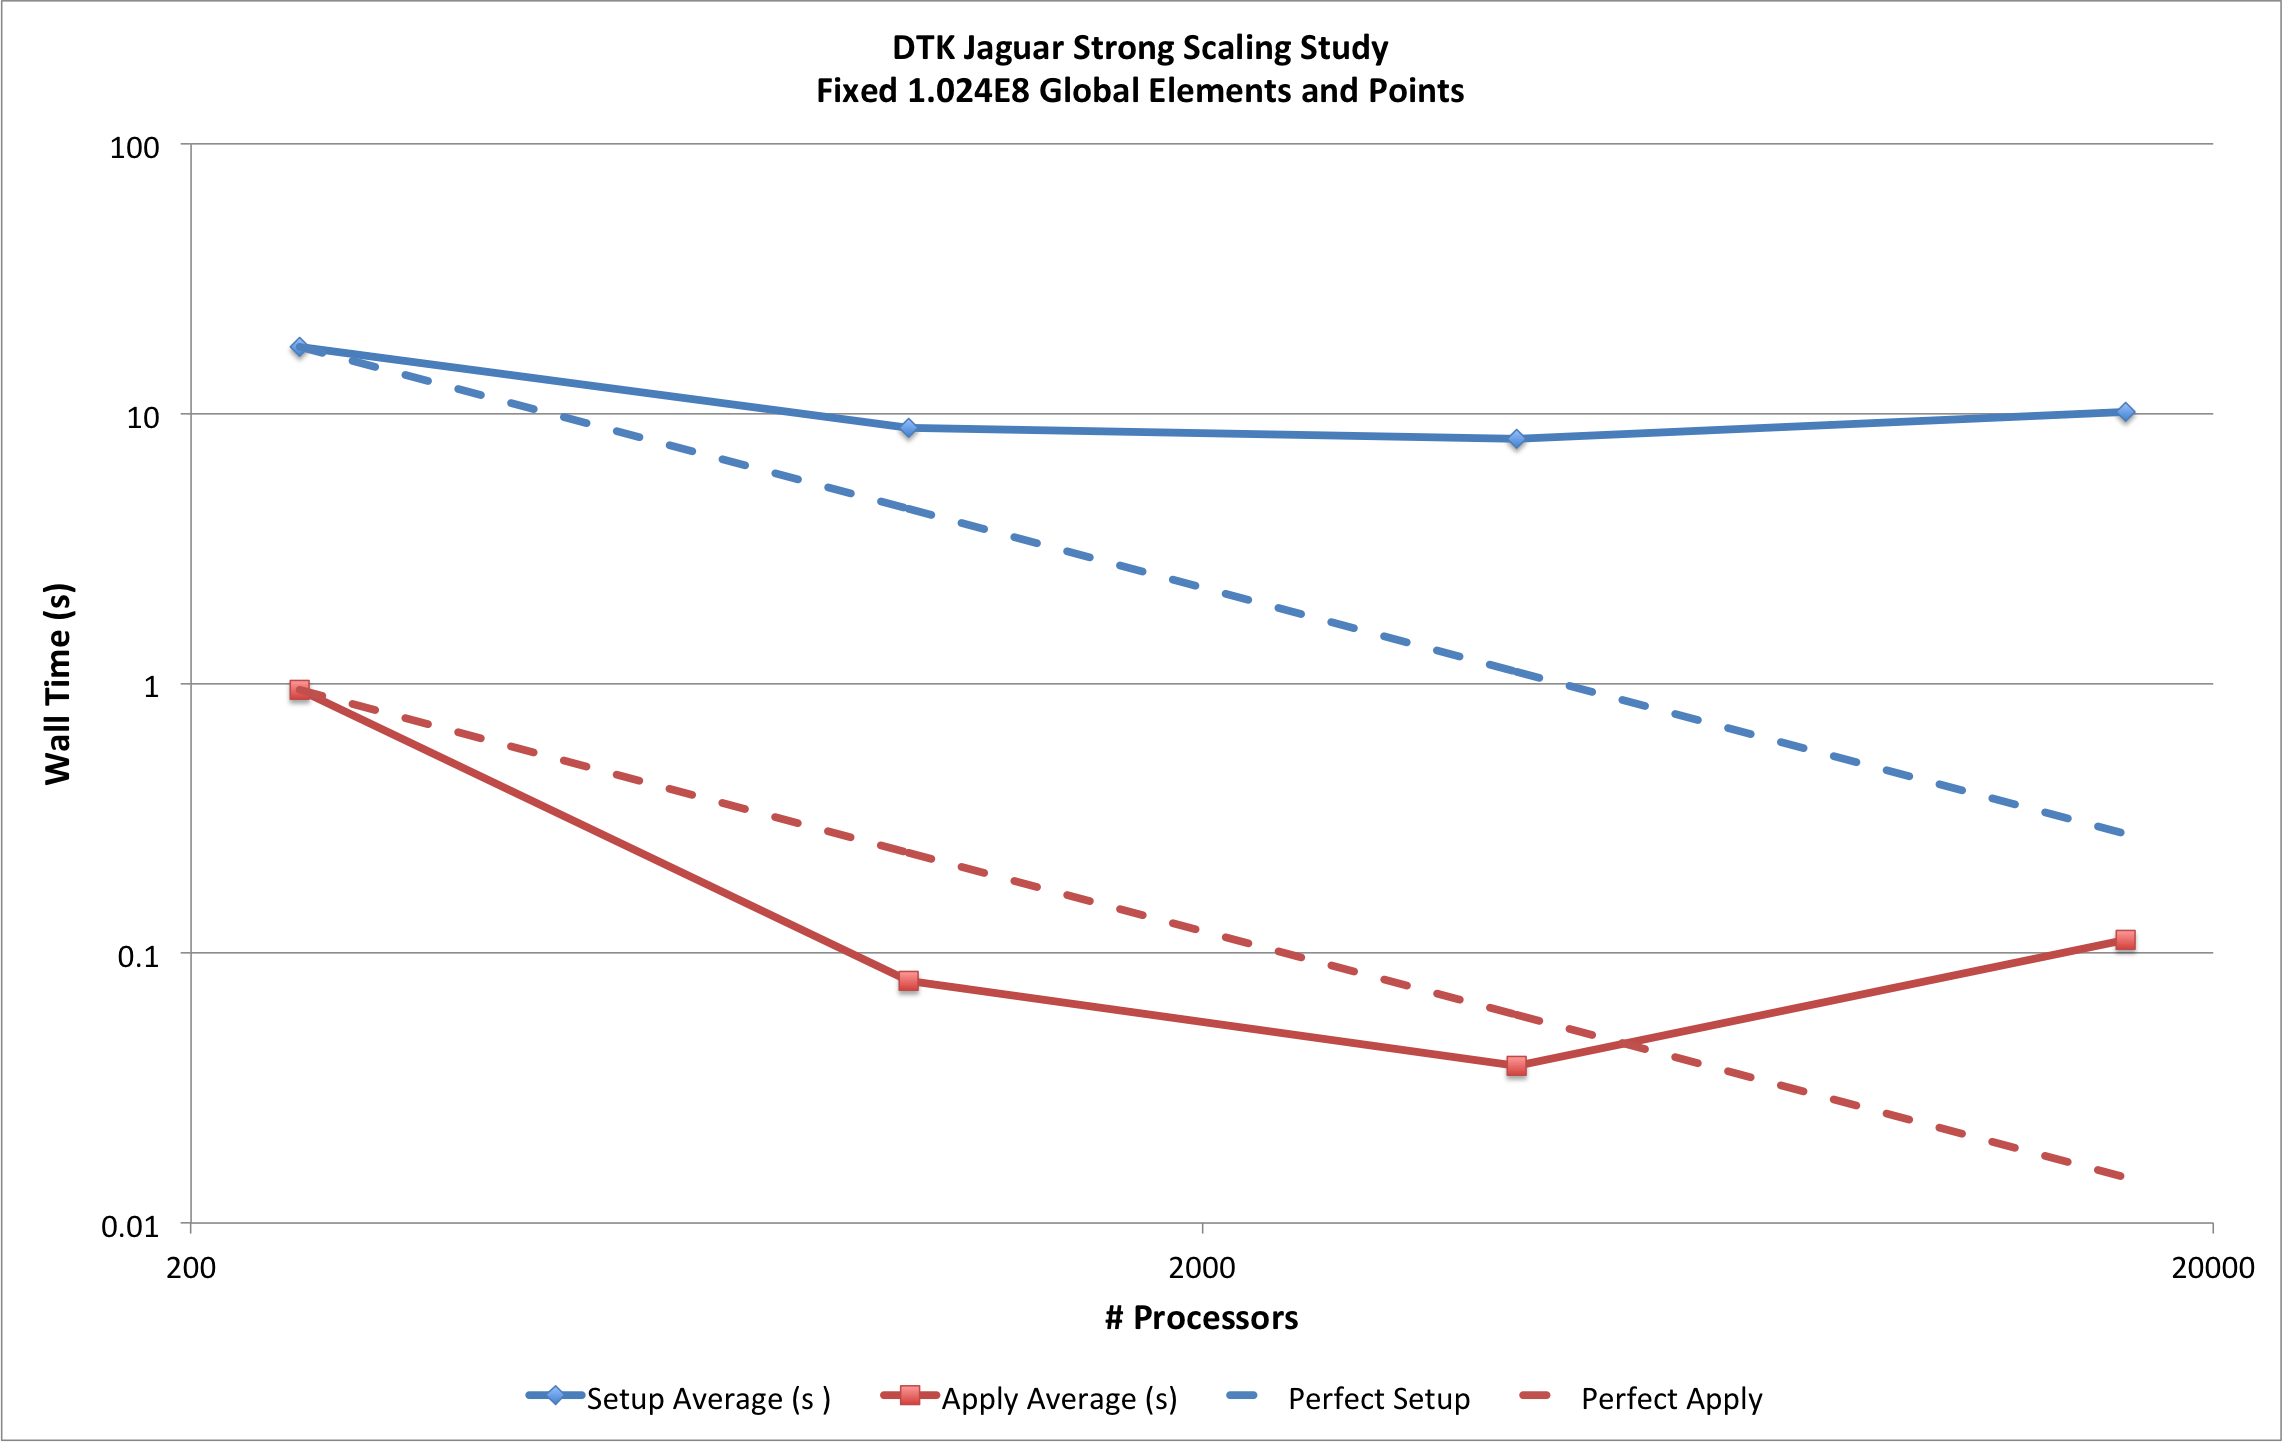
\includegraphics[width=5.5in]{StrongScaling.png}
  \caption{\sl Strong scaling study results with global problem size
    fixed to 1.024E7 elements/points. The blue curve reports the wall
    time to generate the mapping (setup) vs. number of processors
    while the red curve reports the wall time to transfer the data
    (apply) vs. number of processors. The dashed lines give perfect
    strong scaling. Note that the y-axis is a logarithmic scale. }
  \label{fig:strong_scaling}
\end{figure}

\begin{table}[htpb!]
  \begin{center}
    \begin{tabular}{llllllll}\hline\hline
      \multicolumn{1}{l}{}& 
      \multicolumn{1}{l}{Local} & 
      \multicolumn{1}{l}{Setup} & 
      \multicolumn{1}{l}{Setup} & 
      \multicolumn{1}{l}{Setup} & 
      \multicolumn{1}{l}{Apply} & 
      \multicolumn{1}{l}{Apply} & 
      \multicolumn{1}{l}{Apply}\\
      \multicolumn{1}{l}{Procs} & 
      \multicolumn{1}{l}{Elements} & 
      \multicolumn{1}{l}{Min (s)} & 
      \multicolumn{1}{l}{Max (s)} & 
      \multicolumn{1}{l}{Average (s)} & 
      \multicolumn{1}{l}{Min (s)} & 
      \multicolumn{1}{l}{Max (s)} & 
      \multicolumn{1}{l}{Average (s)}\\ \hline\hline
      %%
256 &	4.00E+04 & 17.66 &	17.77 &	17.748 & 0.93 &	0.96 &	0.944 \\
1024 &	1.00E+04 & 8.35 &	8.92 &	8.877 &	0.07 &	0.09 &	0.079 \\
4096 &	2.50E+03 & 7.02 &	8.14 &	8.067 &	0.03 &	0.05 &	0.038 \\
16384 &	6.25E+02 & 6.23 &	10.52 &	10.202 & 0 &	0.03 &	0.112 \\
      \hline\hline
    \end{tabular}
  \end{center}
  \caption{\sl Strong scaling study data. All times reported in
    seconds. Minimum, maximum, and average timing values are global
    and computed using the results from all processes.}
  \label{tab:strong_scaling}
\end{table}

\begin{table}[htpb!]
  \begin{center}
    \begin{tabular}{lll}\hline\hline
      \multicolumn{1}{c}{Procs}& 
      \multicolumn{1}{c}{Setup Efficiency} & 
      \multicolumn{1}{c}{Apply Efficiency}\\\hline\hline
      %%
      1024 &	0.498 &	2.984 \\
      4096 &	0.136 &	1.545 \\
      16384 &	0.026 &	0.131 \\
      \hline\hline
    \end{tabular}
  \end{center}
  \caption{\sl Strong scaling efficiencies. The 16 process case was used
    as the reference case.}
  \label{tab:strong_efficiency}
\end{table}

Again, compared to the work of Plimpton and his colleagues, this weak
scaling behavior for this type of problem is expected (see figure 6 in
the reference).  At a large enough number of processors, the bandwidth
limitations force the wall time to increase as the number of cores is
increased. As expected, this bandwidth limiting behavior is observed
at a larger problem size and number of cores than was observed in 2004
due to the improved computational resources available.

%%---------------------------------------------------------------------------%%
\section{Fixed Number of Processors}
To briefly assess the amount of on-process work that would be required
for the algorithm to exhibit desirable scaling properties, the number
of cores was fixed and the problem size increased. With a fixed number
of cores at 16,384, the number of global hexahedrons and points were
varied from 1.64E8 to 1.48E9 to assess the effect on latency as
compute time was increased. Figure~\ref{fig:fixed_proc} gives the
results of this study. We see that as the number of elements and
random points per partition is increased, wall time responds
linearly. We expect this as although the number of on-process
operations increases (most likely due to the Newton iterations
required for point-in-element queries) and the number of messages sent
in the communication is fixed, the amount of data communicated
increases as well. Table~\ref{tab:fixed_proc} gives the raw data for
this study.

\begin{figure}[htpb!]
  \centering
  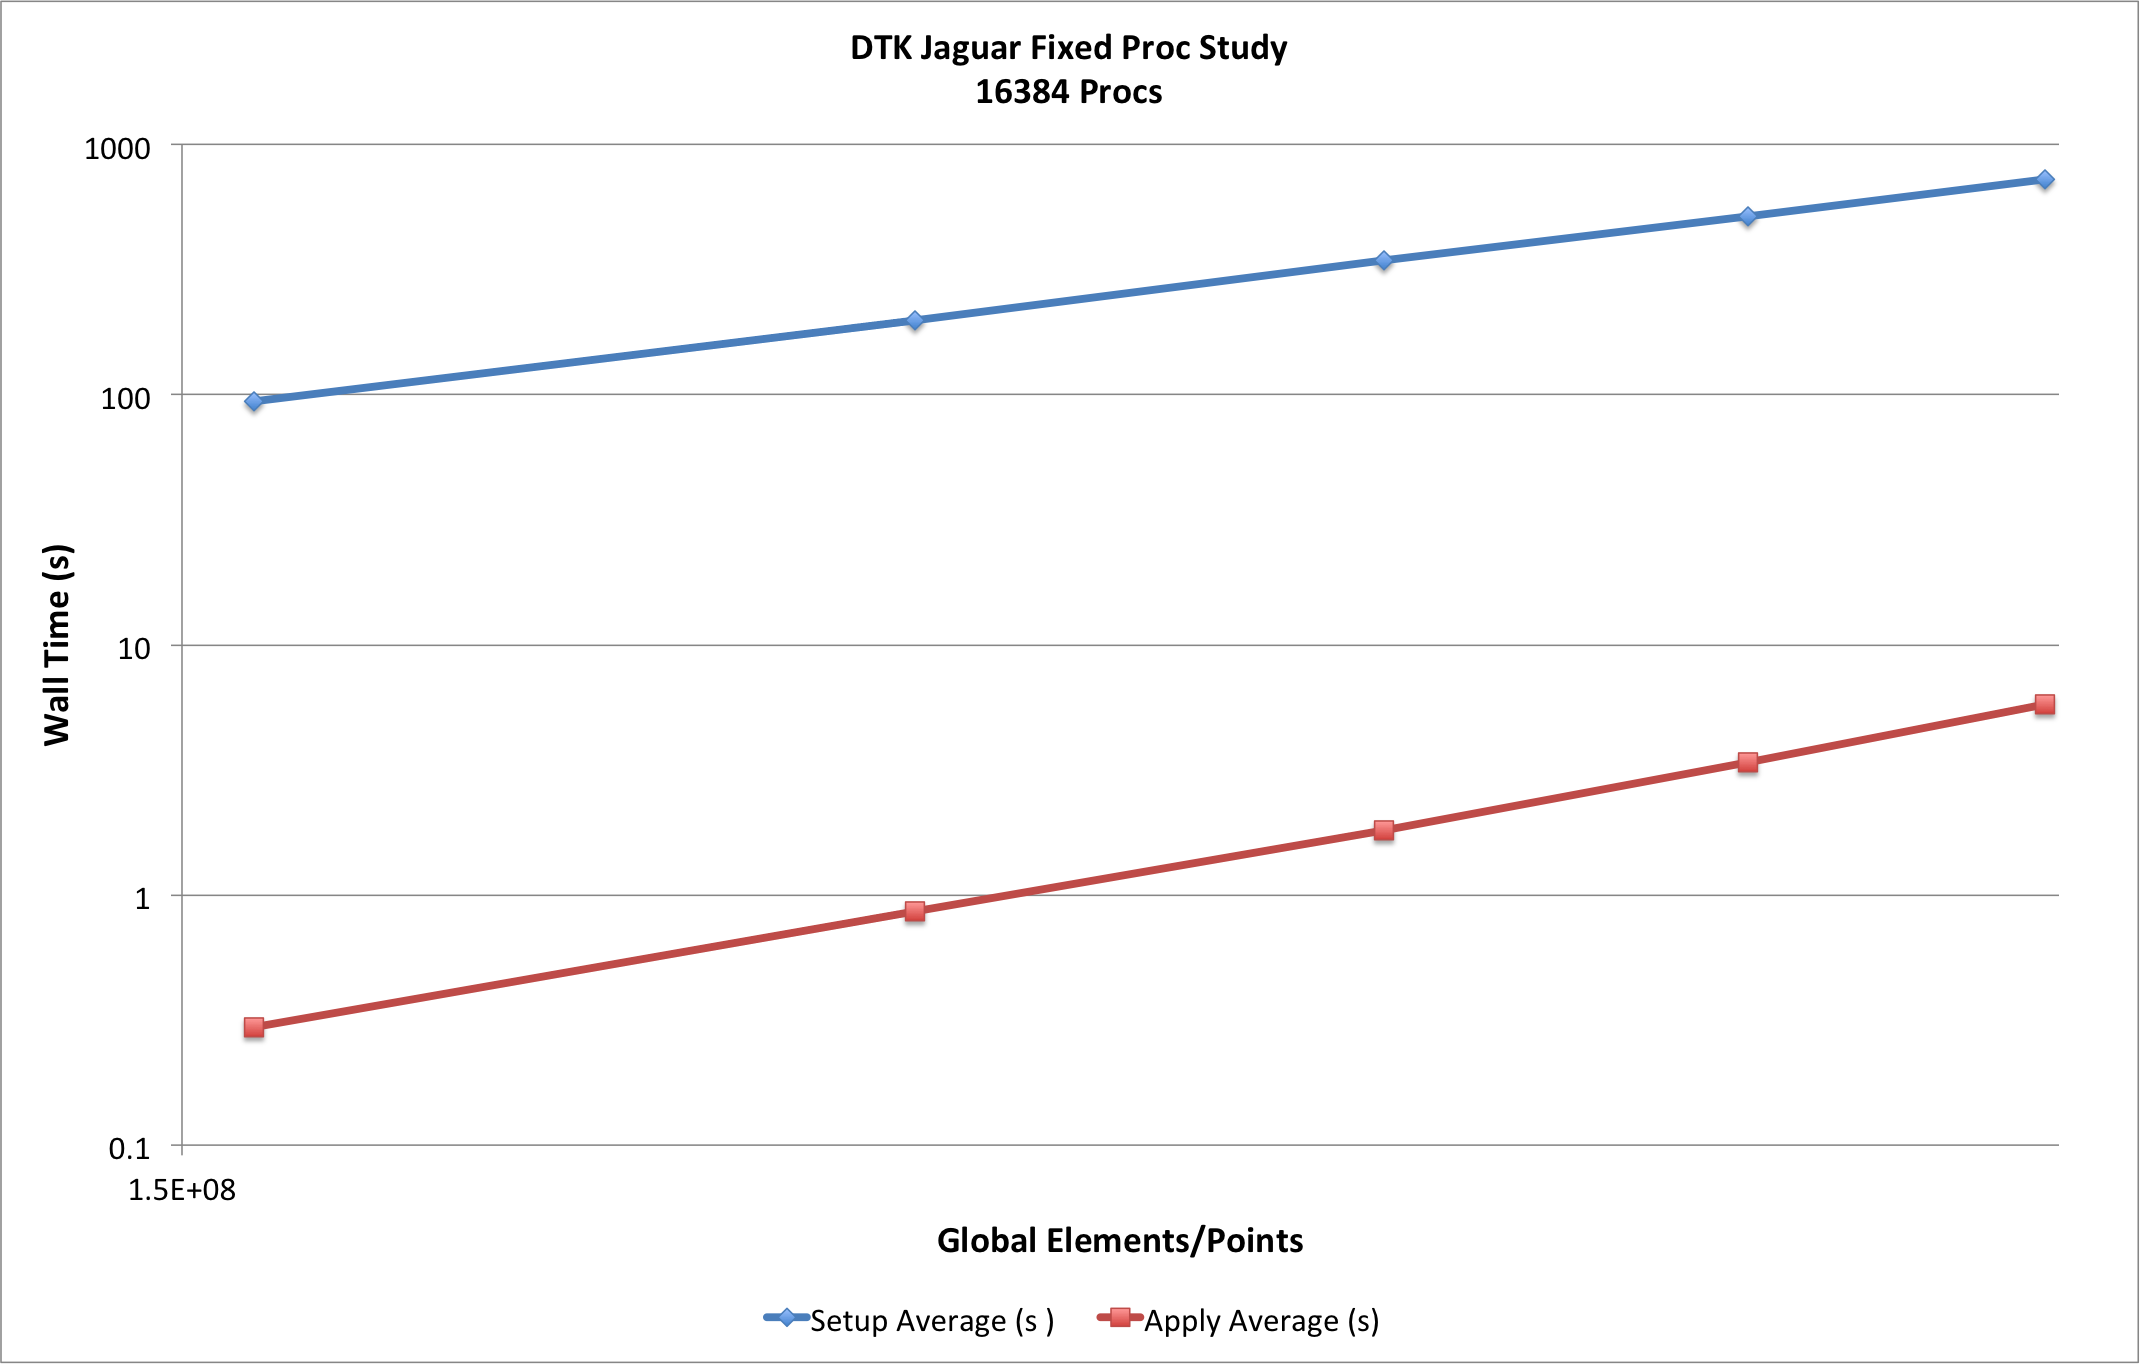
\includegraphics[width=5.5in]{FixedProc.png}
  \caption{\sl Fixed number of processors study results with the
    number of processors fixed at 16,384. The blue curve reports the
    wall time to generate the mapping (setup) vs. number of processors
    while the red curve reports the wall time to transfer the data
    (apply) vs. number of processors. Note that both axis are on a
    logarithmic scale. }
  \label{fig:fixed_proc}
\end{figure}

\begin{table}[htpb!]
  \begin{center}
    \begin{tabular}{lllllll}\hline\hline
      \multicolumn{1}{l}{Global} & 
      \multicolumn{1}{l}{Setup} & 
      \multicolumn{1}{l}{Setup} & 
      \multicolumn{1}{l}{Setup} & 
      \multicolumn{1}{l}{Apply} & 
      \multicolumn{1}{l}{Apply} & 
      \multicolumn{1}{l}{Apply}\\
      \multicolumn{1}{l}{Elements} & 
      \multicolumn{1}{l}{Min (s)} & 
      \multicolumn{1}{l}{Max (s)} & 
      \multicolumn{1}{l}{Average (s)} & 
      \multicolumn{1}{l}{Min (s)} & 
      \multicolumn{1}{l}{Max (s)} & 
      \multicolumn{1}{l}{Average (s)}\\ \hline\hline
      %%
1.6384E+08 & 87.37&	94.93 &	93.915 &	0.28 &	0.32 &	0.296 \\
3.6864E+08 & 188.76 &	198.79 &	197.722 &	0.84 &	0.89 &	0.858 \\
6.5536E+08 & 343.988 &       344.8 &	343.988 & 1.77 &	1.89 &	1.81037 \\
1.0240E+09 & 508.14 &	518.13 &	516.967 &	3.3 &	3.55 &	3.382 \\
      \hline\hline
    \end{tabular}
  \end{center}
  \caption{\sl Fixed number of processors study data. All times
    reported in seconds. Minimum, maximum, and average timing values
    are global and computed using the results from all processes.}
  \label{tab:fixed_proc}
\end{table}

With a maximum problem size of nearly 1.5 billion elements, we see
that a very large problem is required even on 16,384 cores to begin to
overcome some of the latency issues present in the dense communication
problem. However, even for large problems it should be noted that the
wall time is not prohibitively large with approximately 12.5 minutes
needed to setup the 1.5 billion element case. 

%%---------------------------------------------------------------------------%%
\section{Improvements and New Results}
Additional DTK developement has resulted in several implementation
improvements that have provided better performance results and are
therefore reported here. First, it was found in the previous
implementation that generated the results reported above that data was
being discarded during generation of the rendezvous decomposition that
could be used later in the mapping algorithm. Keeping this data
resulted in the elimination of a global communication from the
implementation. Second, it was discovered that all Design-By-Contract
checks were still being performed even with an optimized build. This
feature has been altered such that Design-By-Contract can be toggled
regardless of whether or not the build is debug or optimized.

The new weak scaling study results are presented below in
Figure~\ref{fig:new_weak_scaling} and are compared to the old results
(double dashed line with markers) and the expected behavior for
perfect weak scaling (dashed line without markers). We see first that
the speed-up from eliminating Design-By-Contract checks and a global
communication lets us move the calculations above 100,000 cores. The
largest case reported here uses 115,072 cores and required 10.44
minutes for map generation and 0.48 seconds for data transfer. As a
reference for comparison with the previous implementation, the 65,536
core case took 3.99 minutes for map generation with the new
implementation as compared to 13.61 minutes with the old
implementation. In the weak scaling results, we also see that the
apply operation is effectively beginning to saturate the network with
this dense all-to-all problem. We see very little improvement overall
in the apply operation due to the fact that only a handful of
Design-By-Contract checks were eliminated from the implementation. For
the map operation, we are not yet seeing network saturation signaling
potential room for more improvement in the implementation.


\begin{figure}[h!]
  \centering
  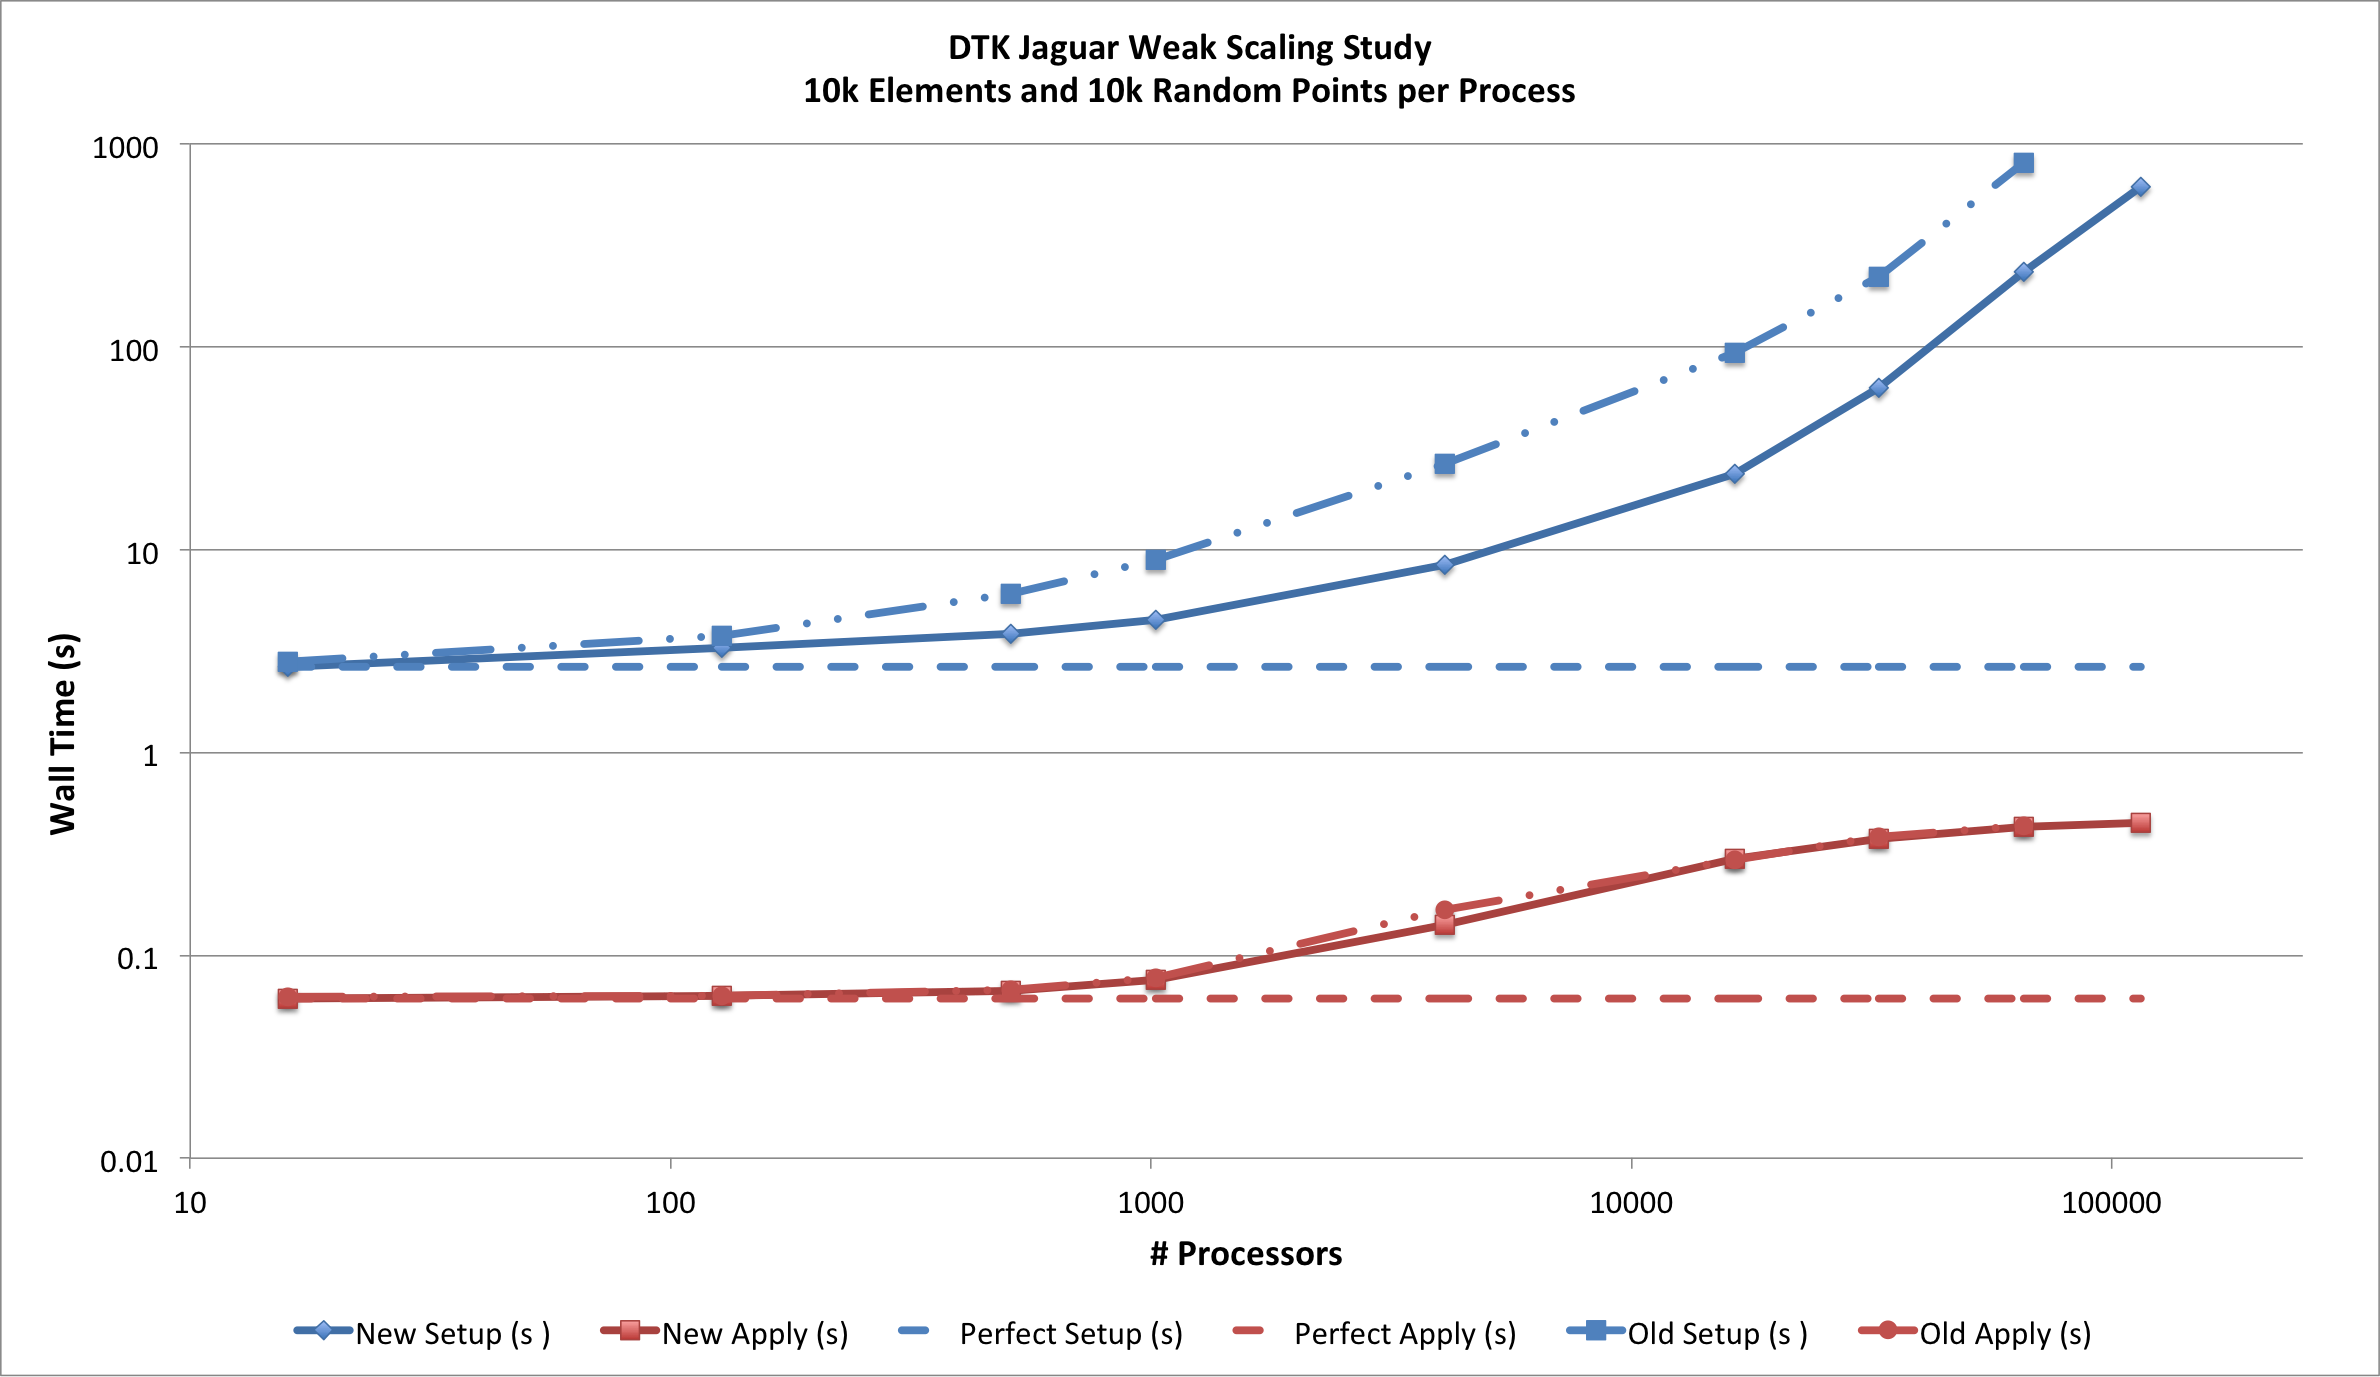
\includegraphics[width=5.5in]{NewWeakScaling.png}
  \caption{\sl New weak scaling study results. The blue curve reports
    the wall time to generate the mapping (setup) vs. number of
    processors while the red curve reports the wall time to transfer
    the data (apply) vs. number of processors. The double-dashed line
    with markers gives the old implementation results and the dashed
    line without markers gives perfect weak scaling behavior. Wall
    time is given in seconds. Note that both axes are on a logarithmic
    scale. }
  \label{fig:new_weak_scaling}
\end{figure}

The strong scaling study was repeated with a larger global problem
size of 1.0E8 elements and points in order to facilitate using larger
numbers of cores. Figure~\ref{fig:new_strong_scaling} gives the
results of these computations. Again we note poor strong scaling in
the setup operation around O(10,000) cores. The strong scaling of the
apply operation has been significantly improved due to the larger
problem size, requiring more data to be computed and
communicated. Given the excellent scaling of the apply operation and
the fact that this is representative of the scaling of the Tpetra
library used for communication, there is hopefully room for
improvement in the setup implementation to improve strong scaling
performance. In addition, a larger problem size may provide better
strong scaling results.

\begin{figure}[htpb!]
  \centering
  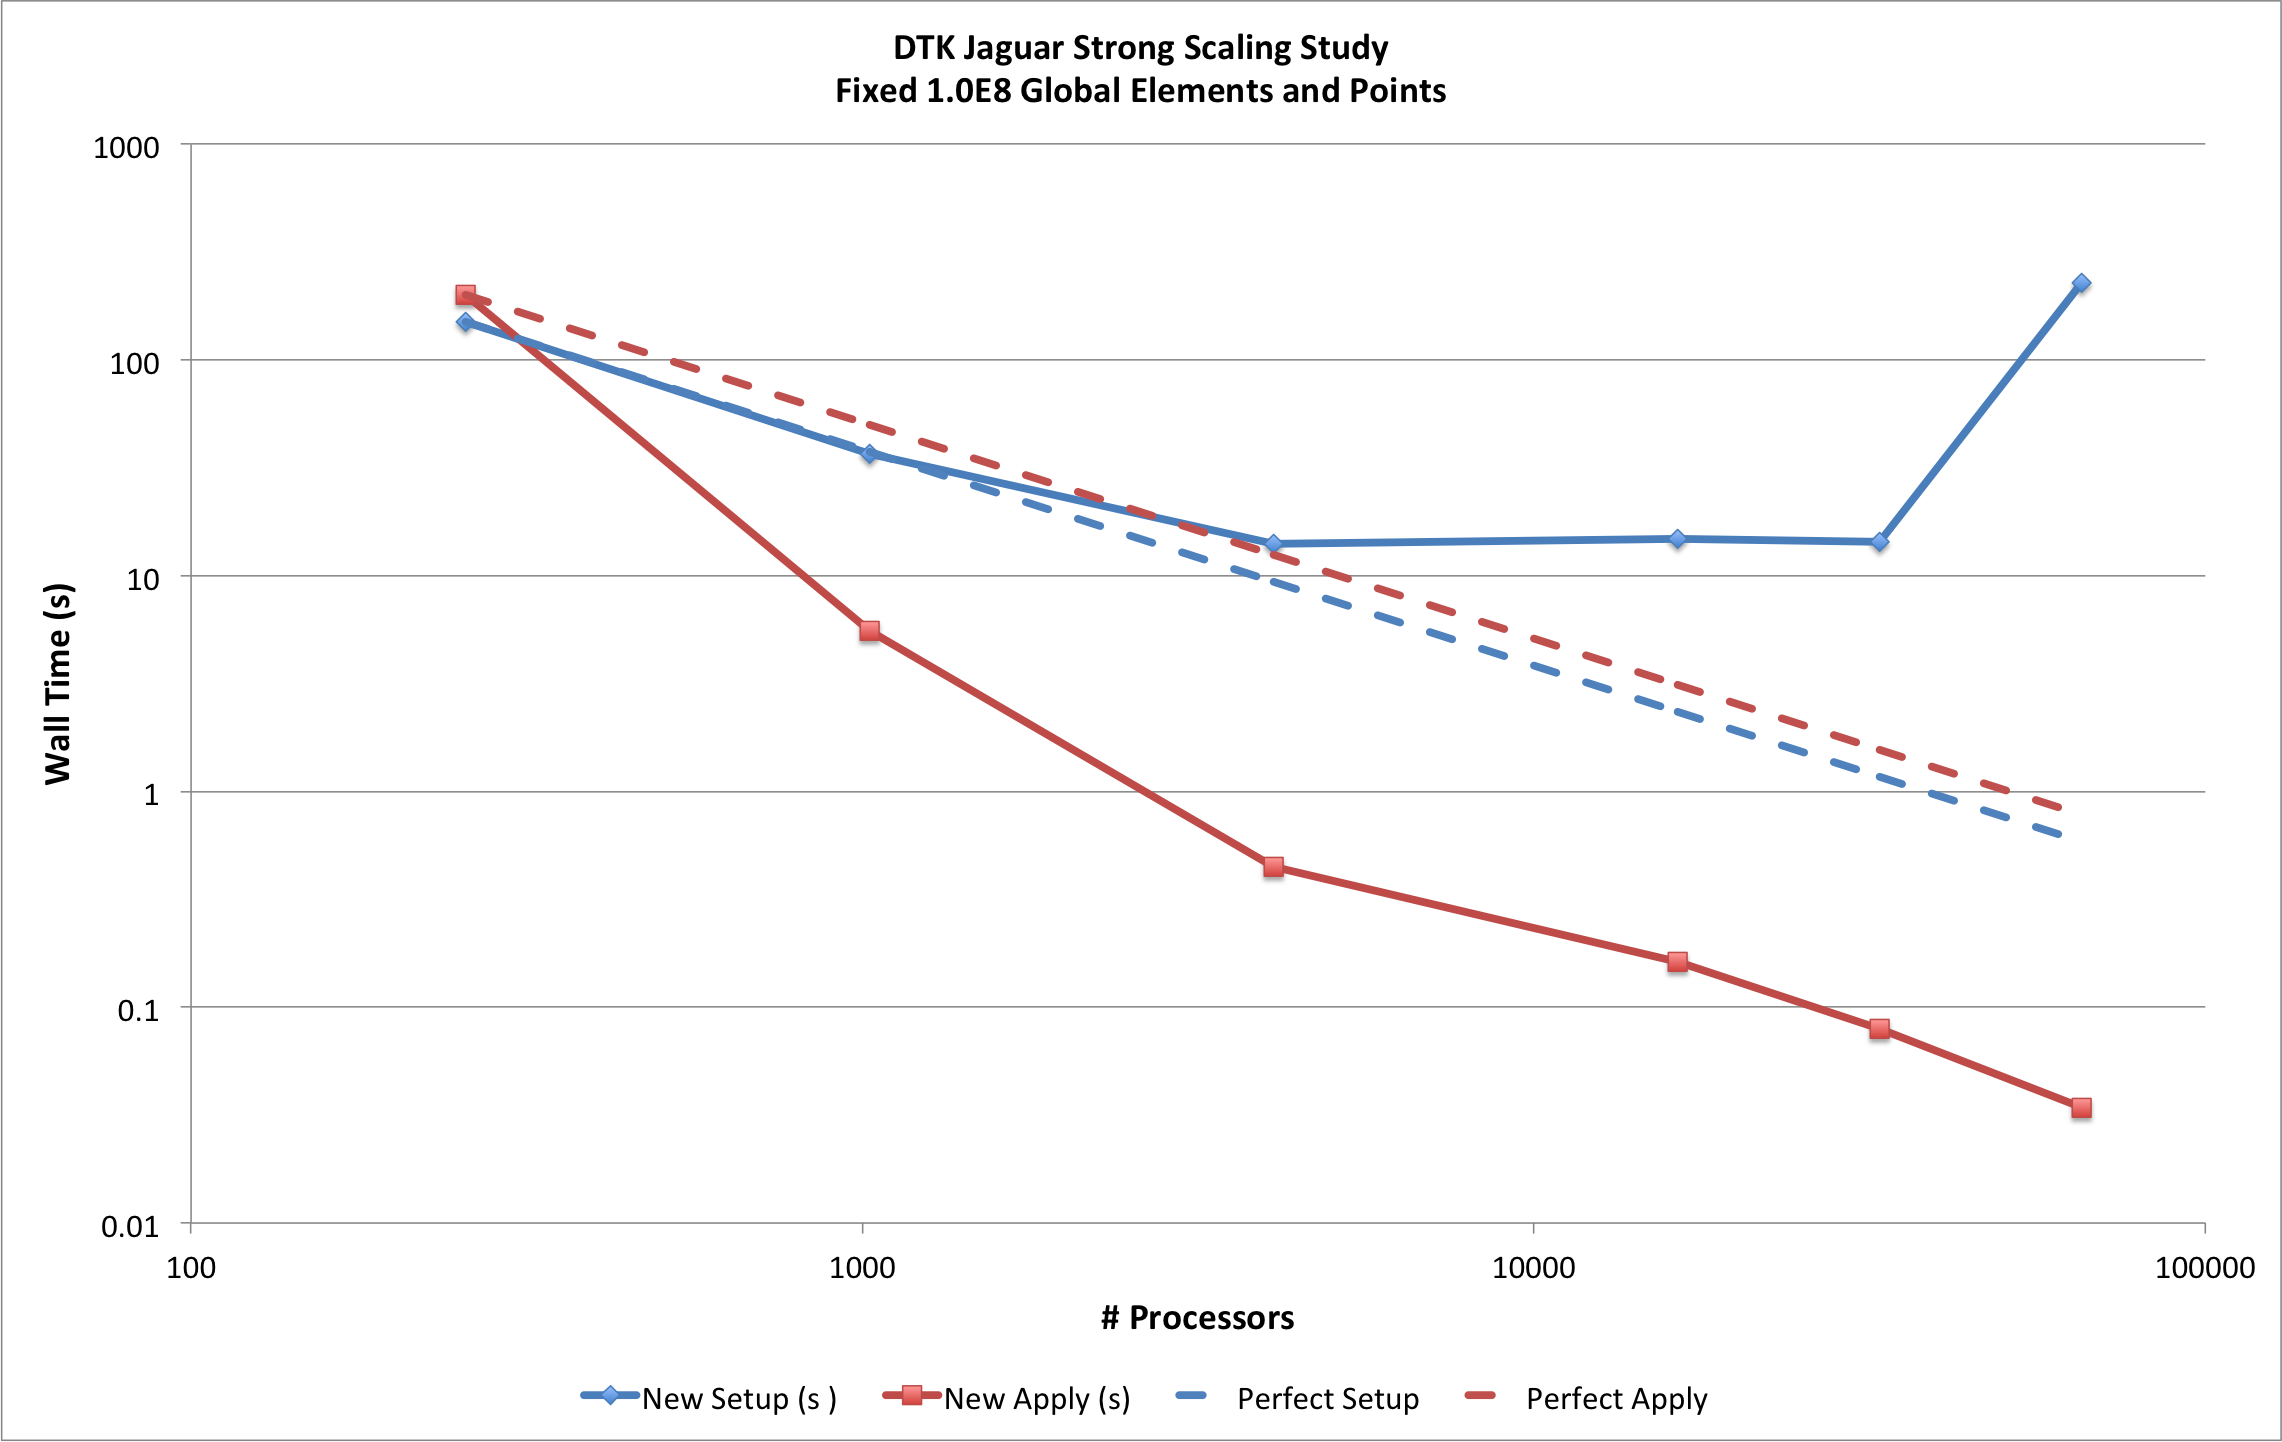
\includegraphics[width=5.5in]{NewStrongScaling.png}
  \caption{\sl New strong scaling study results with global problem
    size fixed to 1.0E8 elements/points. The blue curve reports the
    wall time to generate the mapping (setup) vs. number of processors
    while the red curve reports the wall time to transfer the data
    (apply) vs. number of processors. Perfect strong scaling behavior
    is given by the dashed lines. Wall time is given in seconds. Note
    that the both axes are on a logarithmic scale. }
  \label{fig:new_strong_scaling}
\end{figure}

In addition to renewed weak and strong scaling studies, the largest
fixed processor run from the previous implementation was repeated at
16,384 cores with nearly 1.5 billion elements. Wall time for the setup
operation was reduced from 12.5 minutes to 1.26 minutes with apply
times approximately the same.

%%---------------------------------------------------------------------------%%
\section{Conclusion}
Initial scaling studies have been completed for the Data Transfer Kit
on the Jaguar system. Their results show comparable qualitative
behavior to the literature results with improved performance due to
the more advanced computational resources available. Implementation
improvements have made significant gains in performance, however, for
the dense communication patterns required to complete the scaling
study problem, poor scaling results are still observed above O(10,000)
processors. It is expected for more physical data transfer problems
that the communication pattern will be significantly sparser than the
problem presented here. Because of this, scaling is expected to
improve for more physical problems. Additional scaling studies will be
required to test this hypothesis.

%%---------------------------------------------------------------------------%%
%% BIBLIOGRAPHY STUFF

\bibliographystyle{rnotes}
\bibliography{references}

\closing
\caution
\end{document}

%%---------------------------------------------------------------------------%%
%% end of dtk_scaling_study.tex
%%---------------------------------------------------------------------------%%
